% Preamble:
\documentclass{article}

% Packages:
\usepackage{fancyhdr}
\usepackage{amsmath}
\usepackage{graphicx}
\usepackage{mathbbol}
\usepackage{tikz}
\usetikzlibrary{arrows}
\usetikzlibrary{backgrounds}

% Title Page Information:
\title{CS23 Assignment Five}
\author{CJ Bridgman-Ford \\ cj.ikaika@gmail.com}
\date{April 16, 2024}

% Make subsections lettered:
\renewcommand{\thesubsection}{\alph{subsection}.}

% fancyhdr Page Styling:
\newcommand{\pagenumber}{\thepage\quad}
\newcommand{\authorname}{CJ Bridgman-Ford}

\pagestyle{fancy}
\renewcommand{\headrulewidth}{0pt}
\fancyhead{}
\fancyfoot[L]{\authorname}
\fancyfoot[C]{}
\fancyfoot[R]{\pagenumber}

% End of Preamble.

% Start of document:
\begin{document}

% Title Page:
\maketitle
\thispagestyle{empty}

\clearpage
% Page 1:
\pagenumbering{arabic}

% Problem 1:

\section{We often define graph theory concepts using set theory. For example, given a graph $G=(V,E)$ and a vertex $v \in V$, we define}
\begin{center}
    $N(v) = \{u \in V : \{v,u\}\in E\}$
\end{center}
\section*{\hspace{1cm}We define $N[v]=N(v)\cup\{x\}$. The goal of this problem is to figure out what all this means.}
\subsection{Let $G$ be the graph with $V=\{a,b,c,d,e,f\}$ and $E=\{\{a,b\},\{a,e\},\{b,c\},\{b,e\}.\{c,d\},\{c,f\},\{d,f\},\{e,f\}\}$. Find $N(a)$, $N[a]$, $N(c)$, and $N[c]$.}
\hspace{1cm}\textit{$N(a)=\{b,e\}$, $N[a]=\{a,b,e\}$, $N(c)=\{d,f\}$, and $N[c]=\{c,d,f\}$.}
\subsection{What is the largest and smallest possible values for $|N(v)|$ and $|N[v]|$ for the graph in part (a)? Explain?}
\hspace{1cm}\textit{$a$ has two degrees, $b$ and $c$ each have three, $d$ has two, $e$ has three, and $f$ has only one. Therefore, $|N(v)|$ can be at most $3$ and $|N[v]|$ can be at most $4$. $|N(v)|$ can be at least $2$ and $|N[v]|$ can be at least $1$.}
\subsection{Give an example of a graph $G=(V,E)$ (probably different than the one above) for which $N[v]=V$ for some vertex $v\in V$. Is there a graph for which $N[v]=V$ for all $v \in V$? Explain.}
\hspace{1cm}\textit{Suppose $V = \{a,b,c\}$ and $E = \{\{a,b\},\{a,c\},\{b,c\}\}$. In this case, $N[a]=N[b]=N[c]=\{a,b,c\}$. In this graph, $N[v]=V$ for all vertices $v\in V$.}
\subsection{Give an example of a graph $G=(V,E)$ for which $N(v) = \emptyset$ for some $v\in V$. Is there an example of such a graph for which $N[u]=V$ for some other $u\in V$ as well? Explain.}
\hspace{1cm}\textit{Consider the case where $V=\{a,b,c\}$ and $e=\{b,c\}$. In this case, $N(v)=\emptyset$, as a has a degree of zero.}
\subsection{Describe in words what $N(v)$ and $N[v]$ mean in general.}
\hspace{1cm}\textit{$N(v)$ returns a set of all the nodes that vertex $v$ is directly connected to via an edge. $N[v]$ returns $N(v)\cup\{v\}$, meaning the set of $v$ and all the nodes it connects to.}
\clearpage

% Problem 2:

\section{Which of the following graphs are trees?}
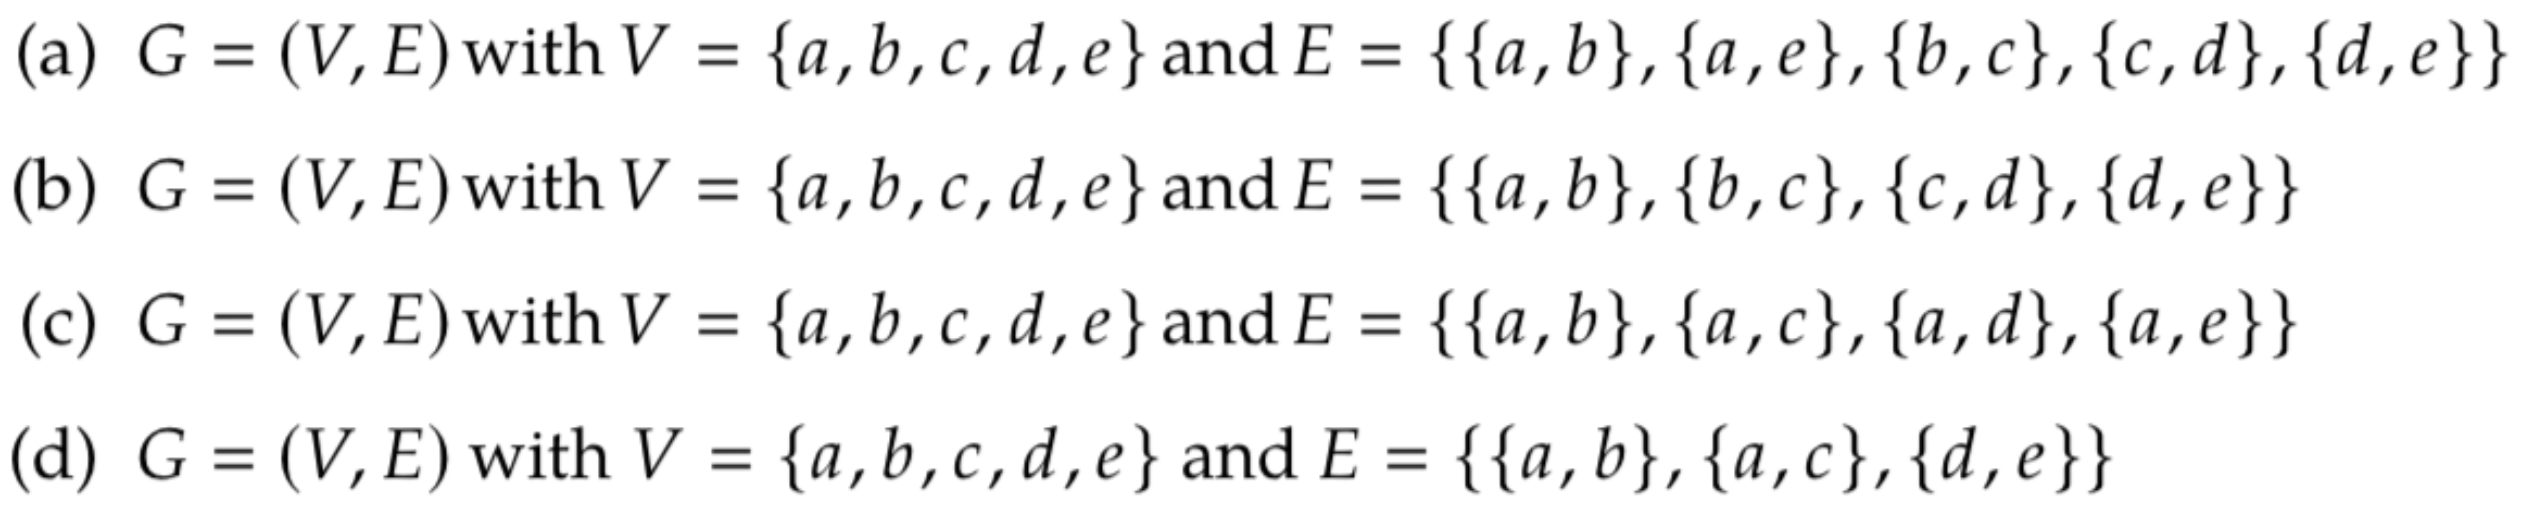
\includegraphics[scale=0.27]{problem2.png} \\

\textit{Trees satisfy two conditions, they do not have cycles and are connected. Graph (a) has a cycle $(a,b,c,d,e,a)$, therefore it is not a tree. Graph (b) is a tree. Graph (c) a tree. Graph (d) is not a tree, as the graph is not fully connected.}



% Problem 3:

\section{For each degree sequence below, decide whether it must always, must never, or could possibly be a degree sequence for a tree.}
\hspace{1cm}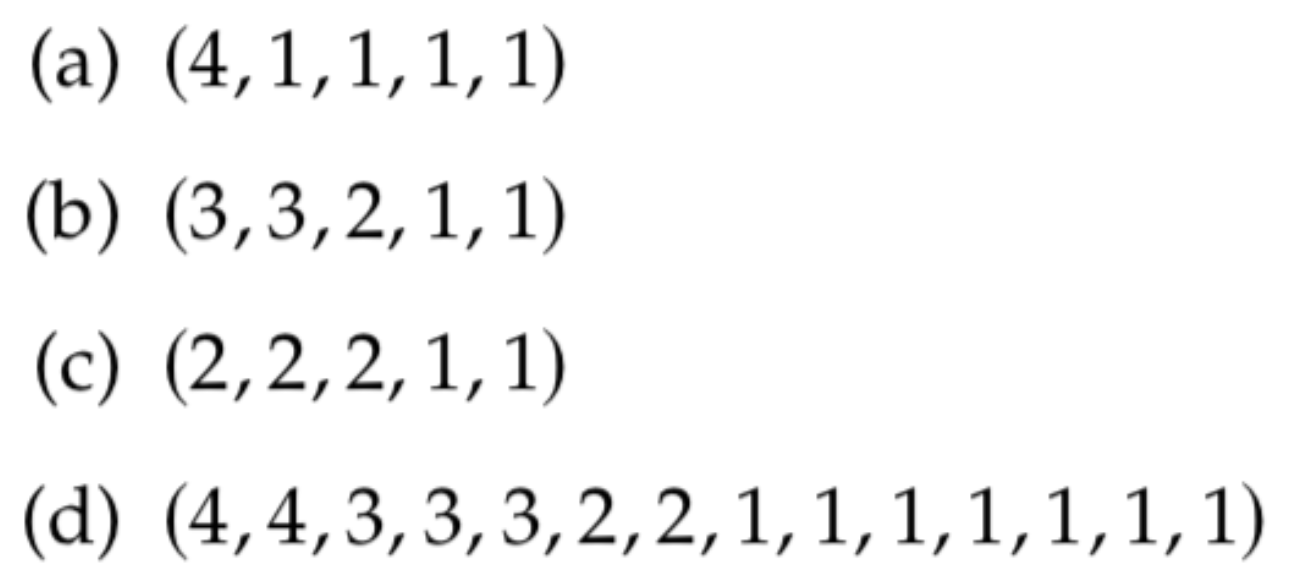
\includegraphics[scale=0.27]{problem3.png}

\textit{For (a), the node degrees must always be a tree. This is evident in problem 2c. For (b), (c), and (d), there's no way to make a tree graph without cycles in it.}

% Problem 4:

\section{Suppose you have a graph with $v$ vertices and $e$ edges that satisfies $v=e+1$. Must the graph be a tree? Prove your answer?}
\textit{The graph could be a tree, but it does not necessarily have to be. Take the graph $V=\{a,b,c,d\}$ with edges $E=\{\{a,b\},\{a,c\},\{b,c\}\}$. The equation is still satisfied, but the graph is not a tree as vertex $d$ has a degree of $0$.}
\clearpage

% Problem 5:

\section{Prove that any graph with $v$ vertices and $e$ edges that satisfies $v>e+1$ will not be connected.}
\hspace{1cm}\textit{Imagine the basic geometric shapes (line | $n=2$, triangle | $n=3$, square | $n=4$, pentagon | $n=5$, etc). In order to completely represent these shapes using a graph, you will need a $n$ vertices and $n$ edges. However, you can still have a connected graph if you take away one edge. This graph will have no cycles, so, for $n$ vertices and $n-1$ edges, you will have a tree graph.}

% Problem 6:

\section{Let $T$ be a rooted tree that contains vertices $u$, $v$, and $w$ (among possibly others). Prove that if $w$ is a descendant of both $u$ and $v$, then $u$ is a descendant of $v$ or vice versa.}
\hspace{1cm}\textit{Since trees do not contain cycles, for a vertex to be a descendant of two other vertices, there must be a traceable path between all three. Suppose the path starts (or the root is) at $u$ and ends and $w$. Then $v$ must be in the middle, making both $v$ and $w$ descendants of $u$. The opposite can be said for the case where the starts at $v$.}

% Problem 7:

\section{Prove that every connected graph which is not itself a tree must have at last three different spanning trees.}

\end{document}